\subsection{Introduction to the Datasets}
\label{data_description}

We will analyse labelling uncertainty in the context of image classification
using the \textit{CIFAR-10H} dataset. The dataset is based on the
\textit{CIFAR-10} (Canadian Institute for Advanced Research, 10 classes)
dataset, first introduced in \cite{Krizhevsky2009LearningML}, which is a
benchmark dataset for image classification and is itself a subset of the larger
\textit{80 million tiny images} dataset, see \cite{torralba80MillionTiny2008}.
The \textit{CIFAR-10} dataset consists of 60'000 images of size $32 \times 32$
pixels. Each image belongs to one of ten classes: airplane, automobile, bird,
cat, deer, dog, frog, horse, ship, and truck. Some example images of each class
are shown in Figure \ref{fig:cifar10example}. The images in the
\textit{CIFAR-10} dataset come with multiple advantages for our purposes, see
\cite{petersonHumanUncertaintyMakes2019}. First, the dataset is well-known and
widely used in the machine learning community, see \cite{PapersCodeCIFAR10} for
a list of papers that use the dataset. Second, the low resolution of the images
makes the dataset challenging for image classification and introduces ambiguity
in the labelling process. Third, the dataset contains images that are close to
the category boundaries, which further introduces ambiguity in the labelling
process. This is in contrast with other datasets that are more carefully created
such that each image is selected to be a unabiguously of a certain
category.\bigskip

\begin{figure}[ht]
  \centering
  \setlength{\tabcolsep}{1pt} % Adjust the space between images
  \renewcommand{\arraystretch}{0} % Adjust the space between rows
  \begin{tabular}{rcccccccccc}
    \textbf{airplane} & \minimagerow{b'airplane'} \\
    \textbf{automobile} & \minimagerow{b'automobile'} \\
    \textbf{bird} & \minimagerow{b'bird'} \\
    \textbf{cat} & \minimagerow{b'cat'} \\
    \textbf{deer} & \minimagerow{b'deer'} \\
    \textbf{dog} & \minimagerow{b'dog'} \\
    \textbf{frog} & \minimagerow{b'frog'} \\
    \textbf{horse} & \minimagerow{b'horse'} \\
    \textbf{ship} & \minimagerow{b'ship'} \\
    \textbf{truck} & \minimagerow{b'truck'}
  \end{tabular}
  \caption{The classes of the CIFAR-10 dataset with ten example images per class.}
  \label{fig:cifar10example}
\end{figure}


The \textit{CIFAR-10} dataset is divided into a training set of 50'000 images
and a test set of 10'000 images. The test set is the basis for the
\textit{CIFAR-10H} dataset, which will be used in this thesis.
\textit{CIFAR-10H} is a balanced dataset, meaning that each class contains the
same number of images, i.e. 1000 images. \textit{CIFAR-10H} is a human-labelled
dataset, where each image has been labelled by multiple human annotators. The
dataset contains 514'200 observations from a total of 2571 annotators. Each
annotator labelled 200 images, 20 from each category, which were randomly
sampled from the test set of the \textit{CIFAR-10} dataset. On average, each
image was labelled 51 times, with the minimum number of labels being 50 and the
maximum number of labels being 63. The relevant features of the
\textit{CIFAR-10H} dataset are described in Table \ref{tab:cifar10hvariables}.
The study design is described in more detail in
\cite{petersonHumanUncertaintyMakes2019}, section 4.2. Note, that the images
where collected based on searching the web, using search engines. Thus, the true
label is not necessarily the object that is displayed in the image, but the term
that was used to search for the image, see \cite{torralba80MillionTiny2008}. For
our purposes, we will assume that the true label is the object that is displayed
in the image.
\bigskip

The \textit{CIFAR-10} and \textit{CIFAR-10H} datasets are publicly available and
can be downloaded from the CIFAR-10 website \cite{CIFAR10CIFAR100Datasetsb} and the
author's GitHub repository \cite{JcpetersonCifar10hOriginal}.

\begin{table}[H]
  \centering
  \begin{tabular}{p{3.5cm}|p{11.5cm}} \textbf{Feature} & \textbf{Description}
  \\
  \hline
  annotator\_id & Unique integer ID ranging from 0 to 2570\\
  \hline
  trial\_index & Indexes the trial for each annotator, from 0 to 219\\
  \hline
  true\_category & True string class name (e.g., "cat") of the image. The set of
  categories is \{airplane, automobile, bird, cat, deer, dog, frog, horse, ship, truck\}\\
  \hline
  chosen\_category & String class name (e.g., "cat") chosen by the
  annotator for the image from the set of possible true categories\\
  \hline
  correct\_guess & Whether the guess was correct (i.e., when
  true\_category == chosen\_category), marked by 1, or 0 otherwise\\
  \hline
  image\_filename & Filename of the PNG (e.g.,
  "cabin\_cruiser\_s\_000814.png")\\
  \hline
  subcategory & Subordinate class label, which is recoverable from the
  image filenames (e.g., "cabin\_cruiser")\\
  \hline
  reaction\_time & Time taken (in milliseconds) by the annotator to provide a
  response for the current trial\\
  \hline
  time\_elapsed & Total time (in milliseconds) that passed at the end of each
  trial. The first is equal to the reaction\_time for the first trial. The rest
  are essentially cumulative reaction\_time values
  \end{tabular}
  \caption{Features of the CIFAR-10H dataset.}
  \label{tab:cifar10hvariables}
\end{table}



\subsection{Descriptive Statistics}
\label{desc_stats}

As mentioned in the previous section, the \textit{CIFAR-10H} dataset is balanced
with respect to the true categories. This means, that we have 51'420
observations per true category. But the number of observations per chosen
category is not balanced, see Figure \ref{fig:chosen_category}, e.g. the
category \textit{deer} is underrepresented, while the category \textit{dog} is
overrepresented. The question that arrises is, whether chosen categories are
usually correct or not and where the votes of overrepresented categories come
from.

\begin{figure}[H]
  \centering
  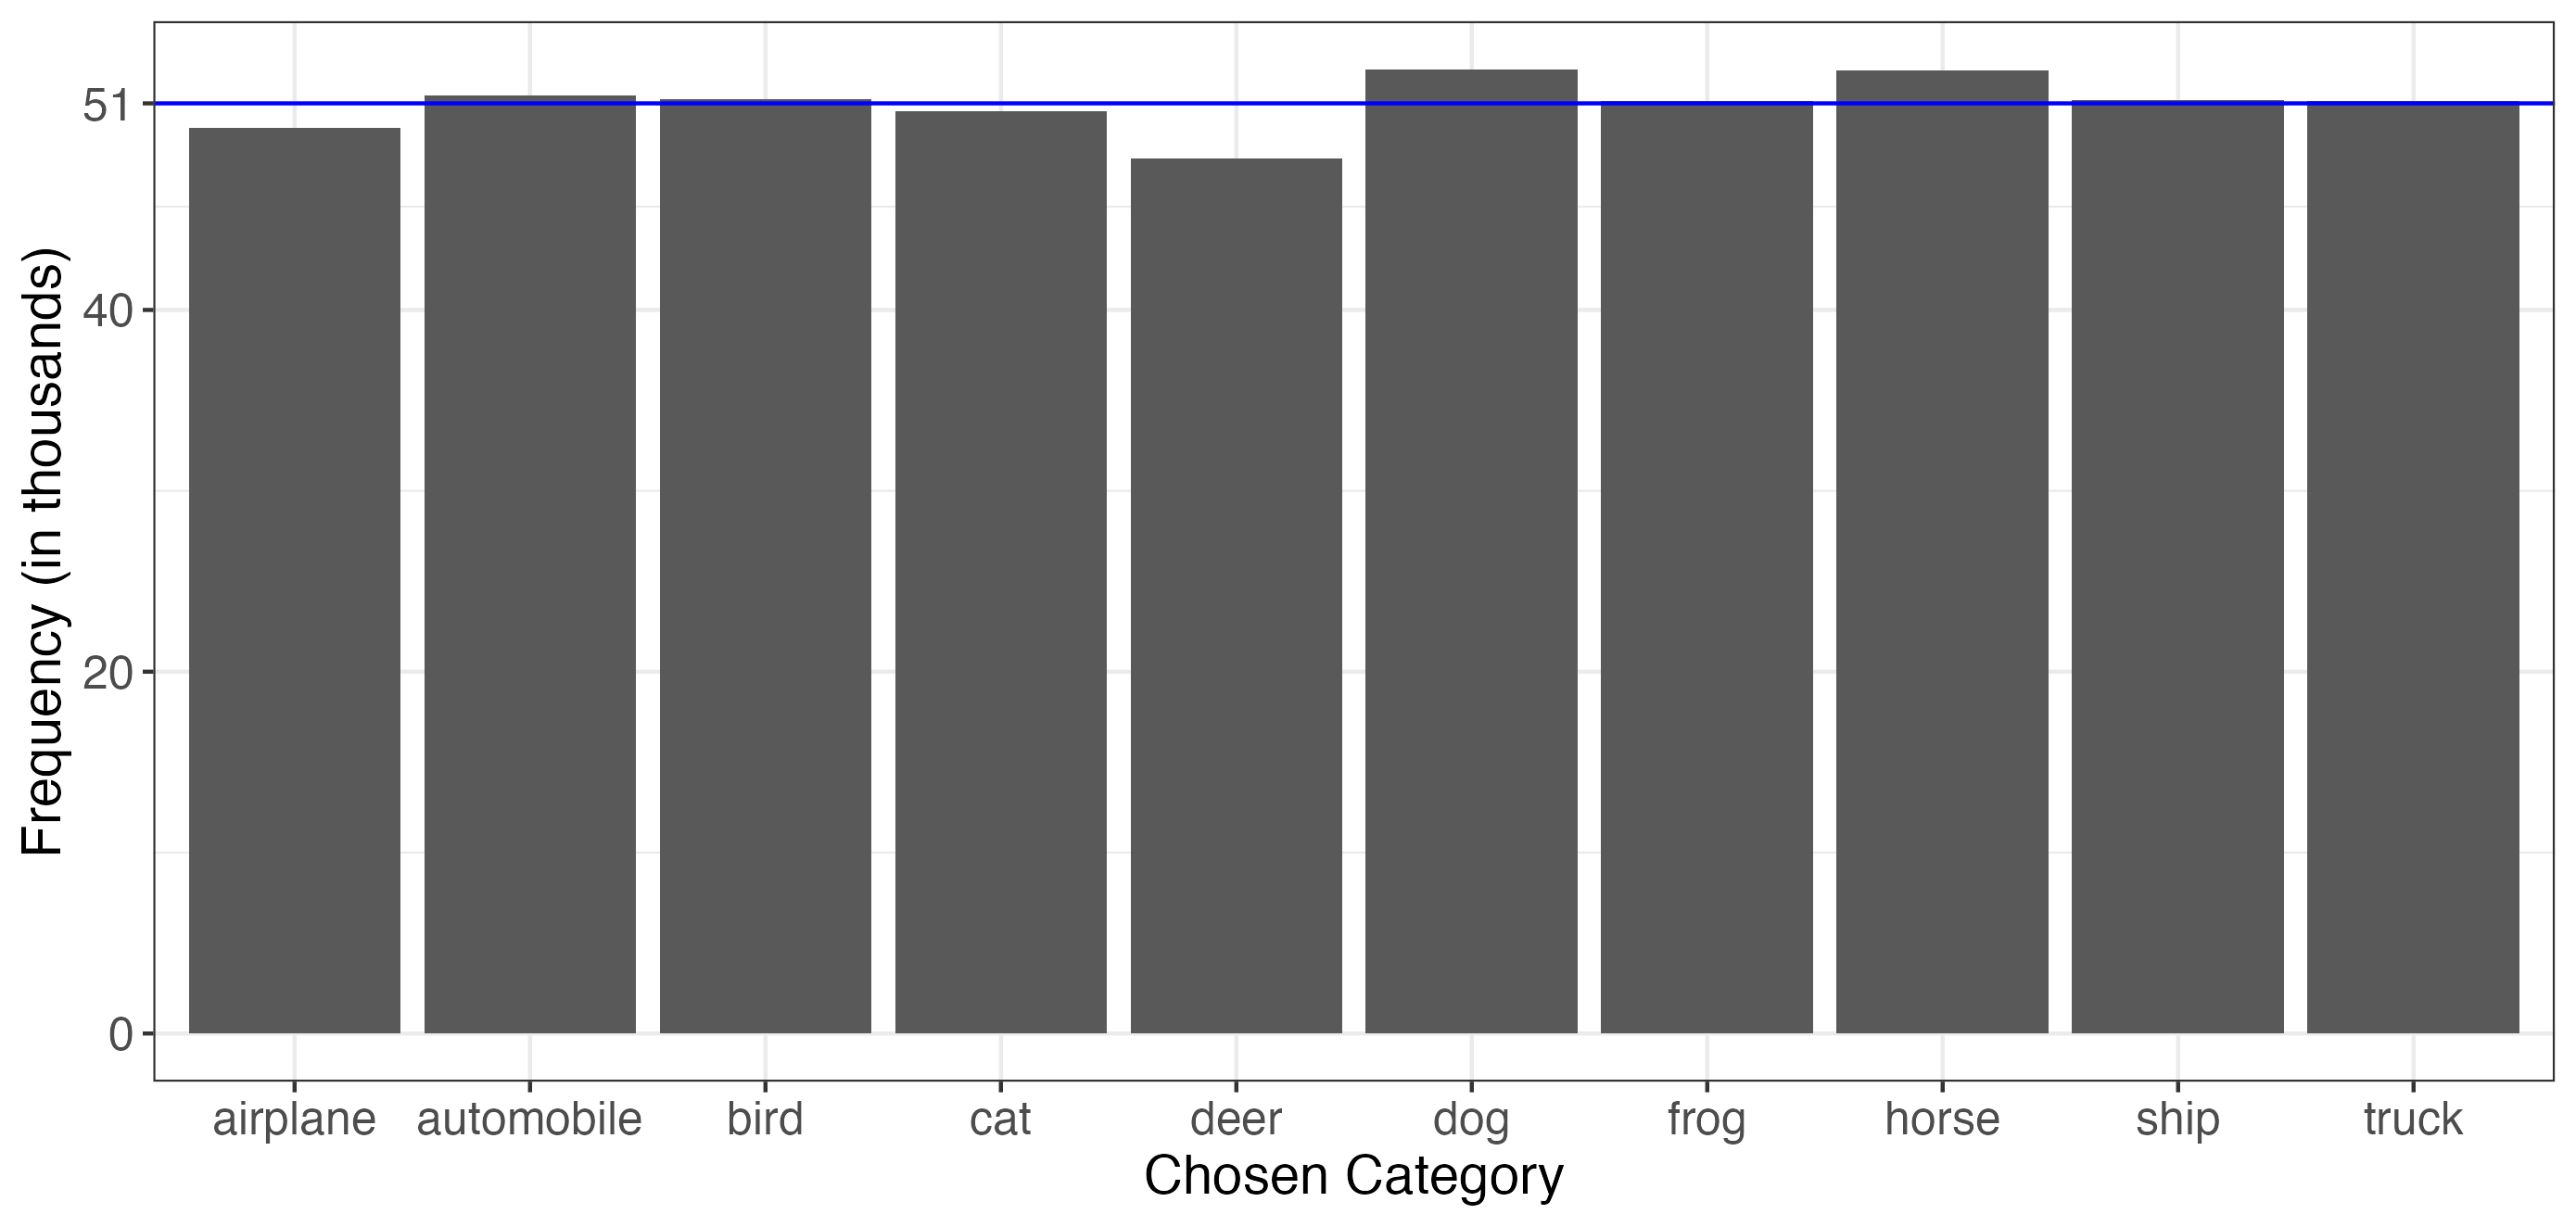
\includegraphics[width = 0.8\textwidth]{../figs/chosen_category.png}
  \caption{Number of observations per chosen category. The blue horizontal line
  indicates the 51'420 observations per true category, so that we can see, which
  categories are over- and underrepresented.}
  \label{fig:chosen_category}
\end{figure}

We can also question the ambiguity of the images. For that, we can check, how
many unique labels each image has received. If an image is unambiguous, then all
annotators should agree on the label of the image. If an image is ambiguous,
then there are multiple possible labels for the image. In Figure
\ref{fig:consensus_distribution}, we can see the distribution of the number of
labels per image for each true category. We can see, that in all categories,
50\% of the images have received at most 2 labels. We can also see, that in
almost all categories, 25\% of the images have received 3 labels or more. This
indicates that a lot of images are unambiguous, but also that a considerable amount of
images are ambiguous.

\begin{figure}[H]
  \centering
  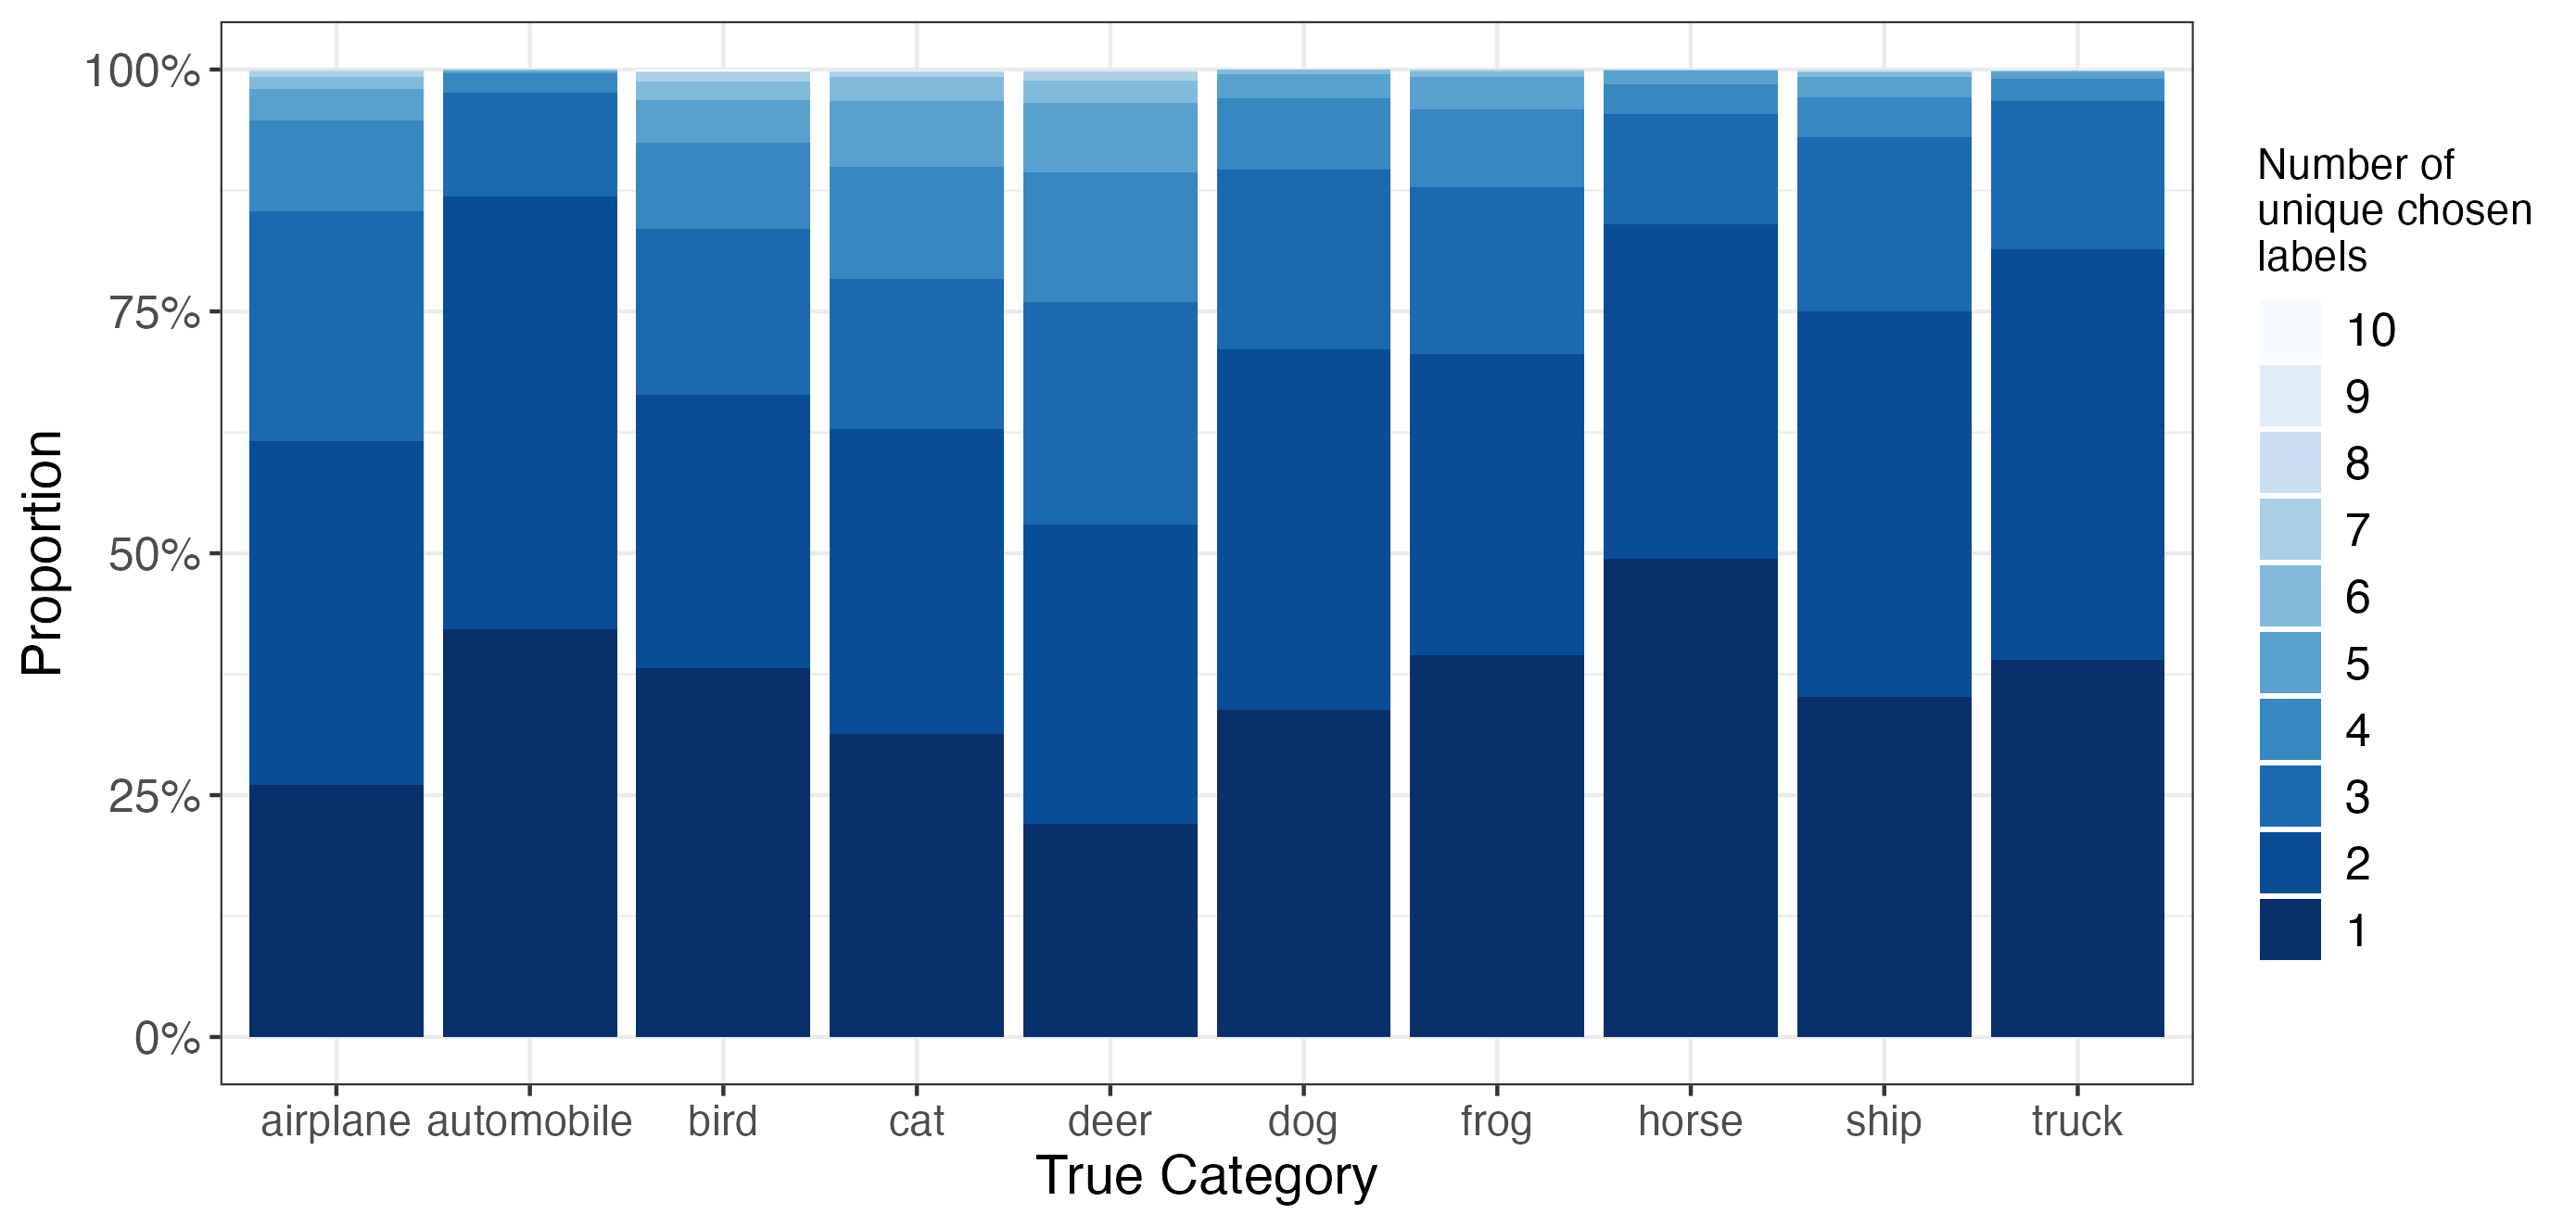
\includegraphics[width = 0.8\textwidth]{../figs/consensus_distribution.png}
  \caption{Distribution of the number of unique chosen labels per image for each true category.
  Unambiguous images have received only one label, while ambiguous images have received multiple labels.
  The more labels an image has received, the more ambiguous the image is.
  }
  \label{fig:consensus_distribution}
\end{figure}

In Figure \ref{fig:ambiguous_image}, we can see an examples of ambiguous and
unambiguous images as well as their respective vote distribution.

\begin{figure}[ht]
  \centering
  \setlength{\tabcolsep}{1pt} % Adjust the space between images
  \renewcommand{\arraystretch}{0} % Adjust the space between rows
  \begin{tabular}{ccc}
    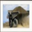
\includegraphics[width = 0.3\textwidth]{../figs/cifar_images_examples/ambiguous_image2.png} & 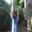
\includegraphics[width = 0.3\textwidth]{../figs/cifar_images_examples/ambiguous_image1.png} & 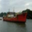
\includegraphics[width = 0.3\textwidth]{../figs/cifar_images_examples/unambiguous_image.png} \\
    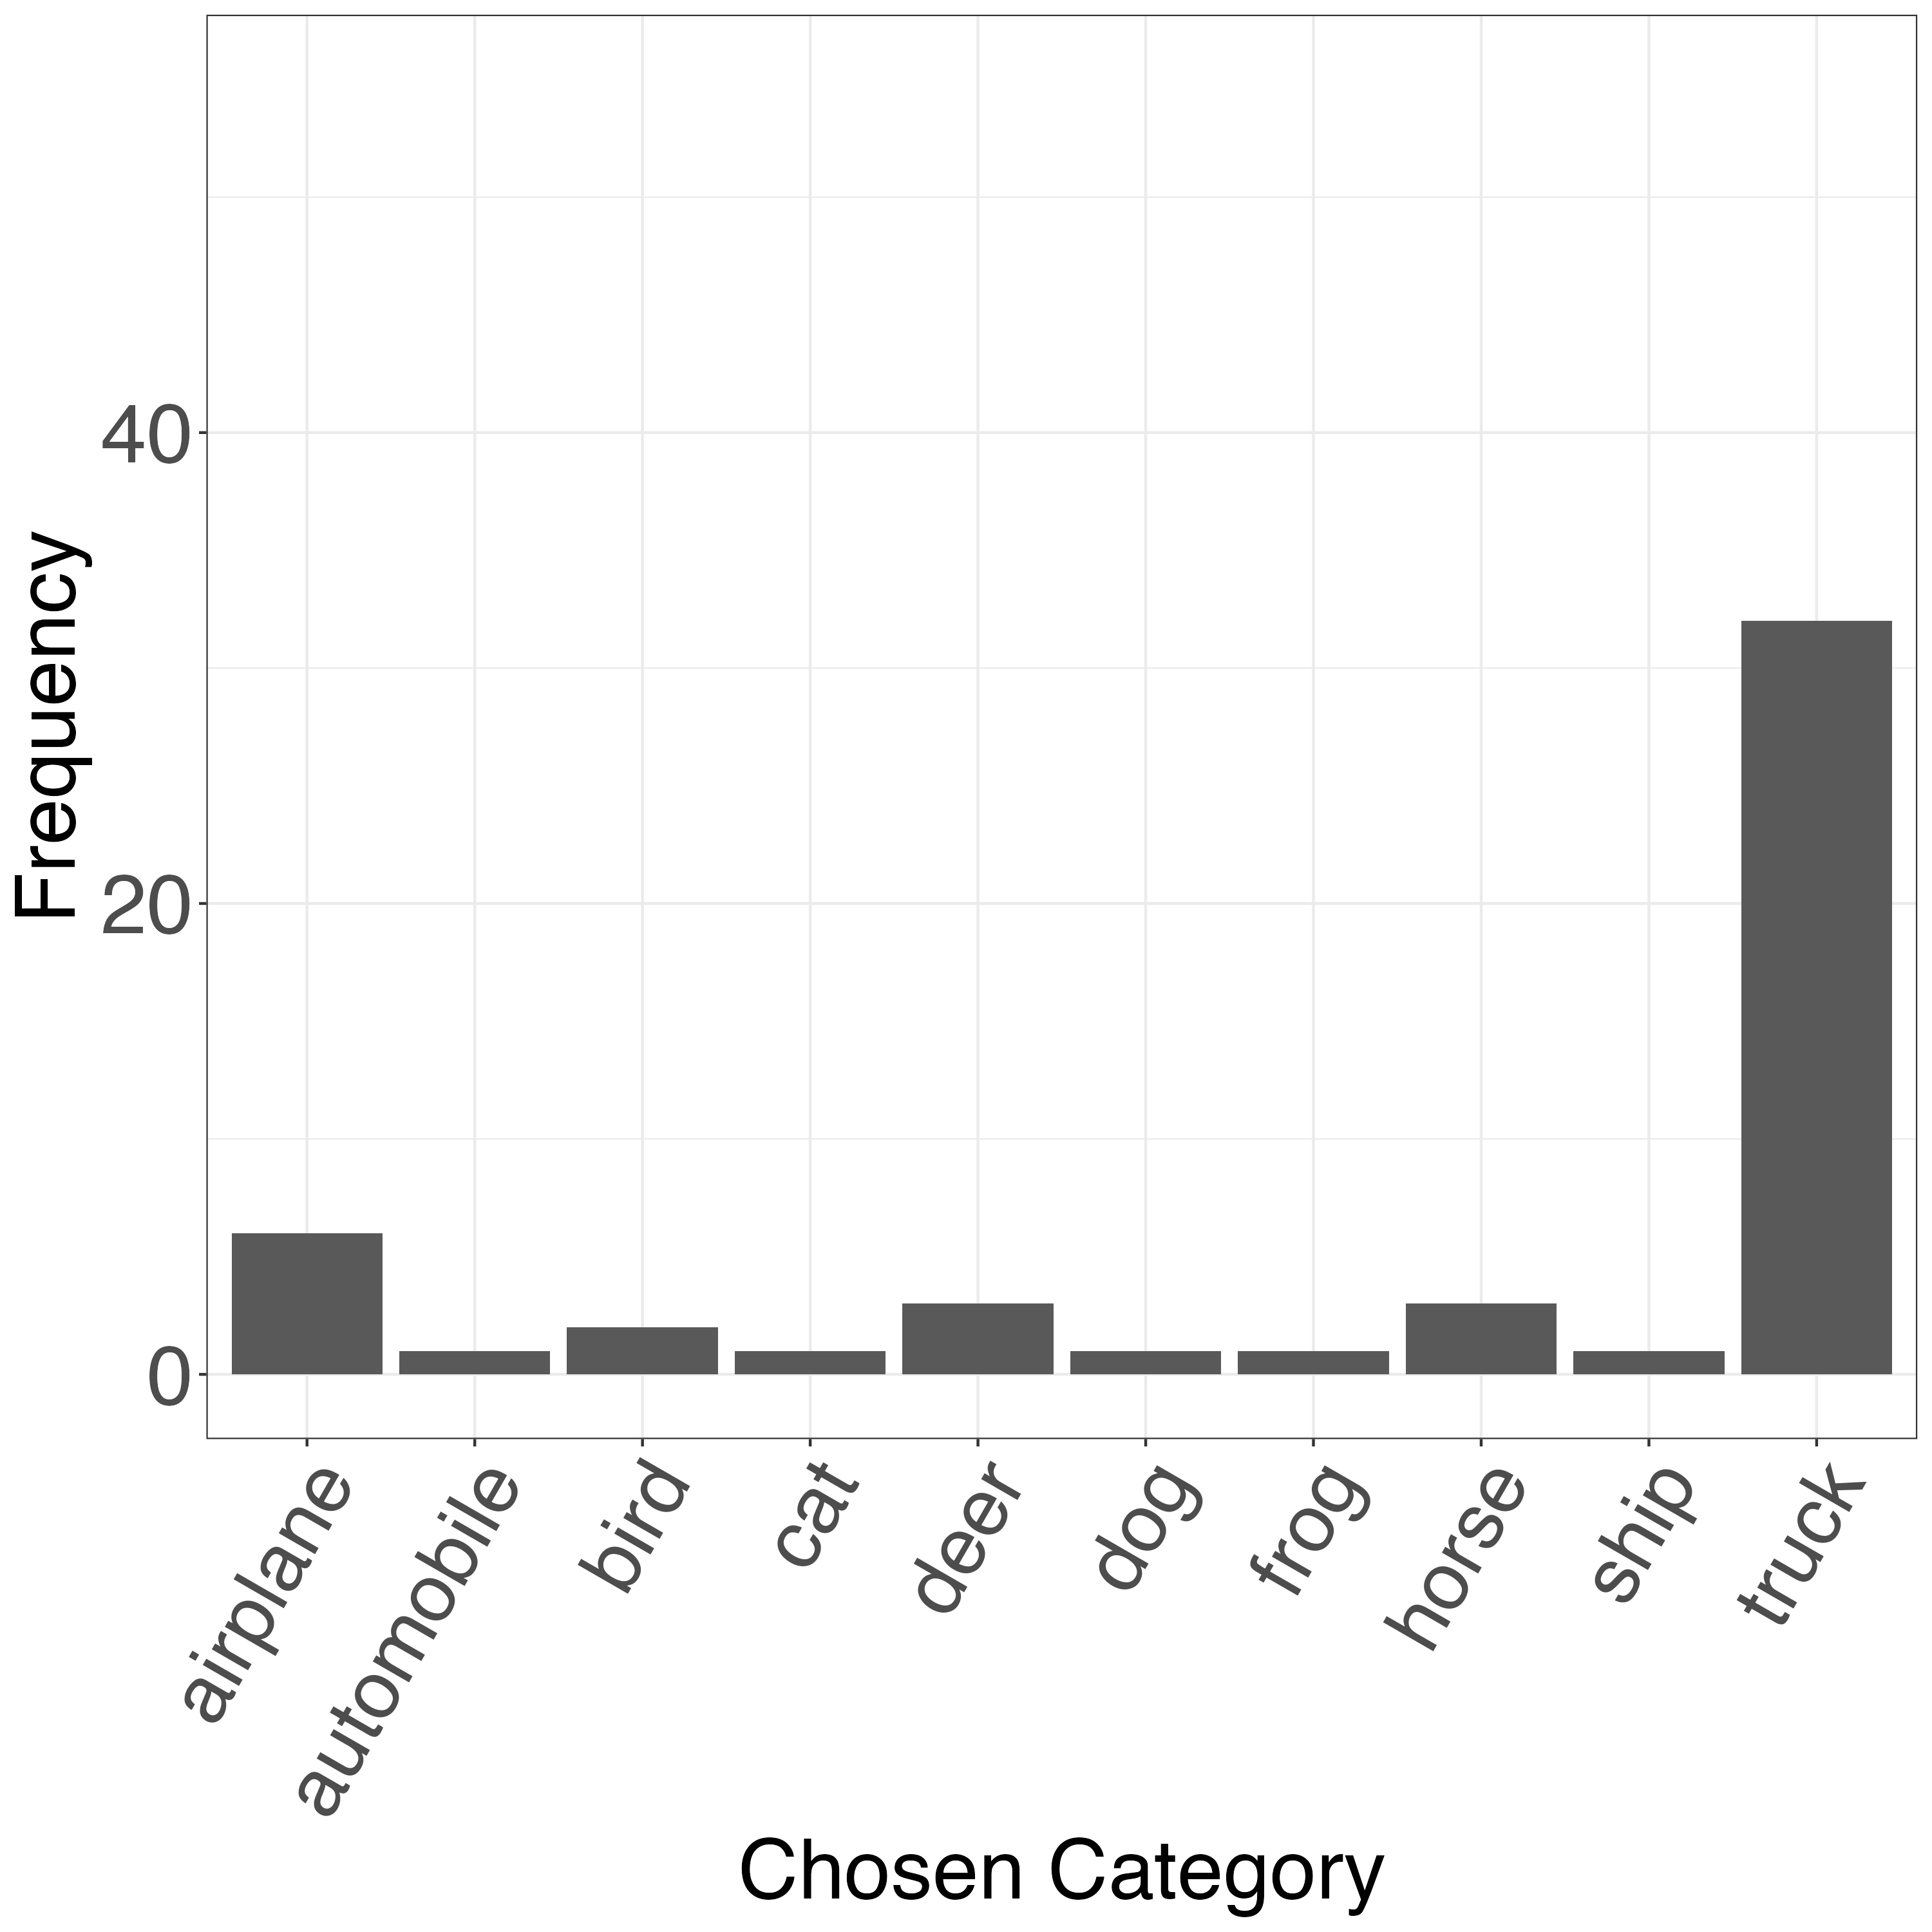
\includegraphics[width = 0.3\textwidth]{../figs/ambiguous_image1_dist.png} & 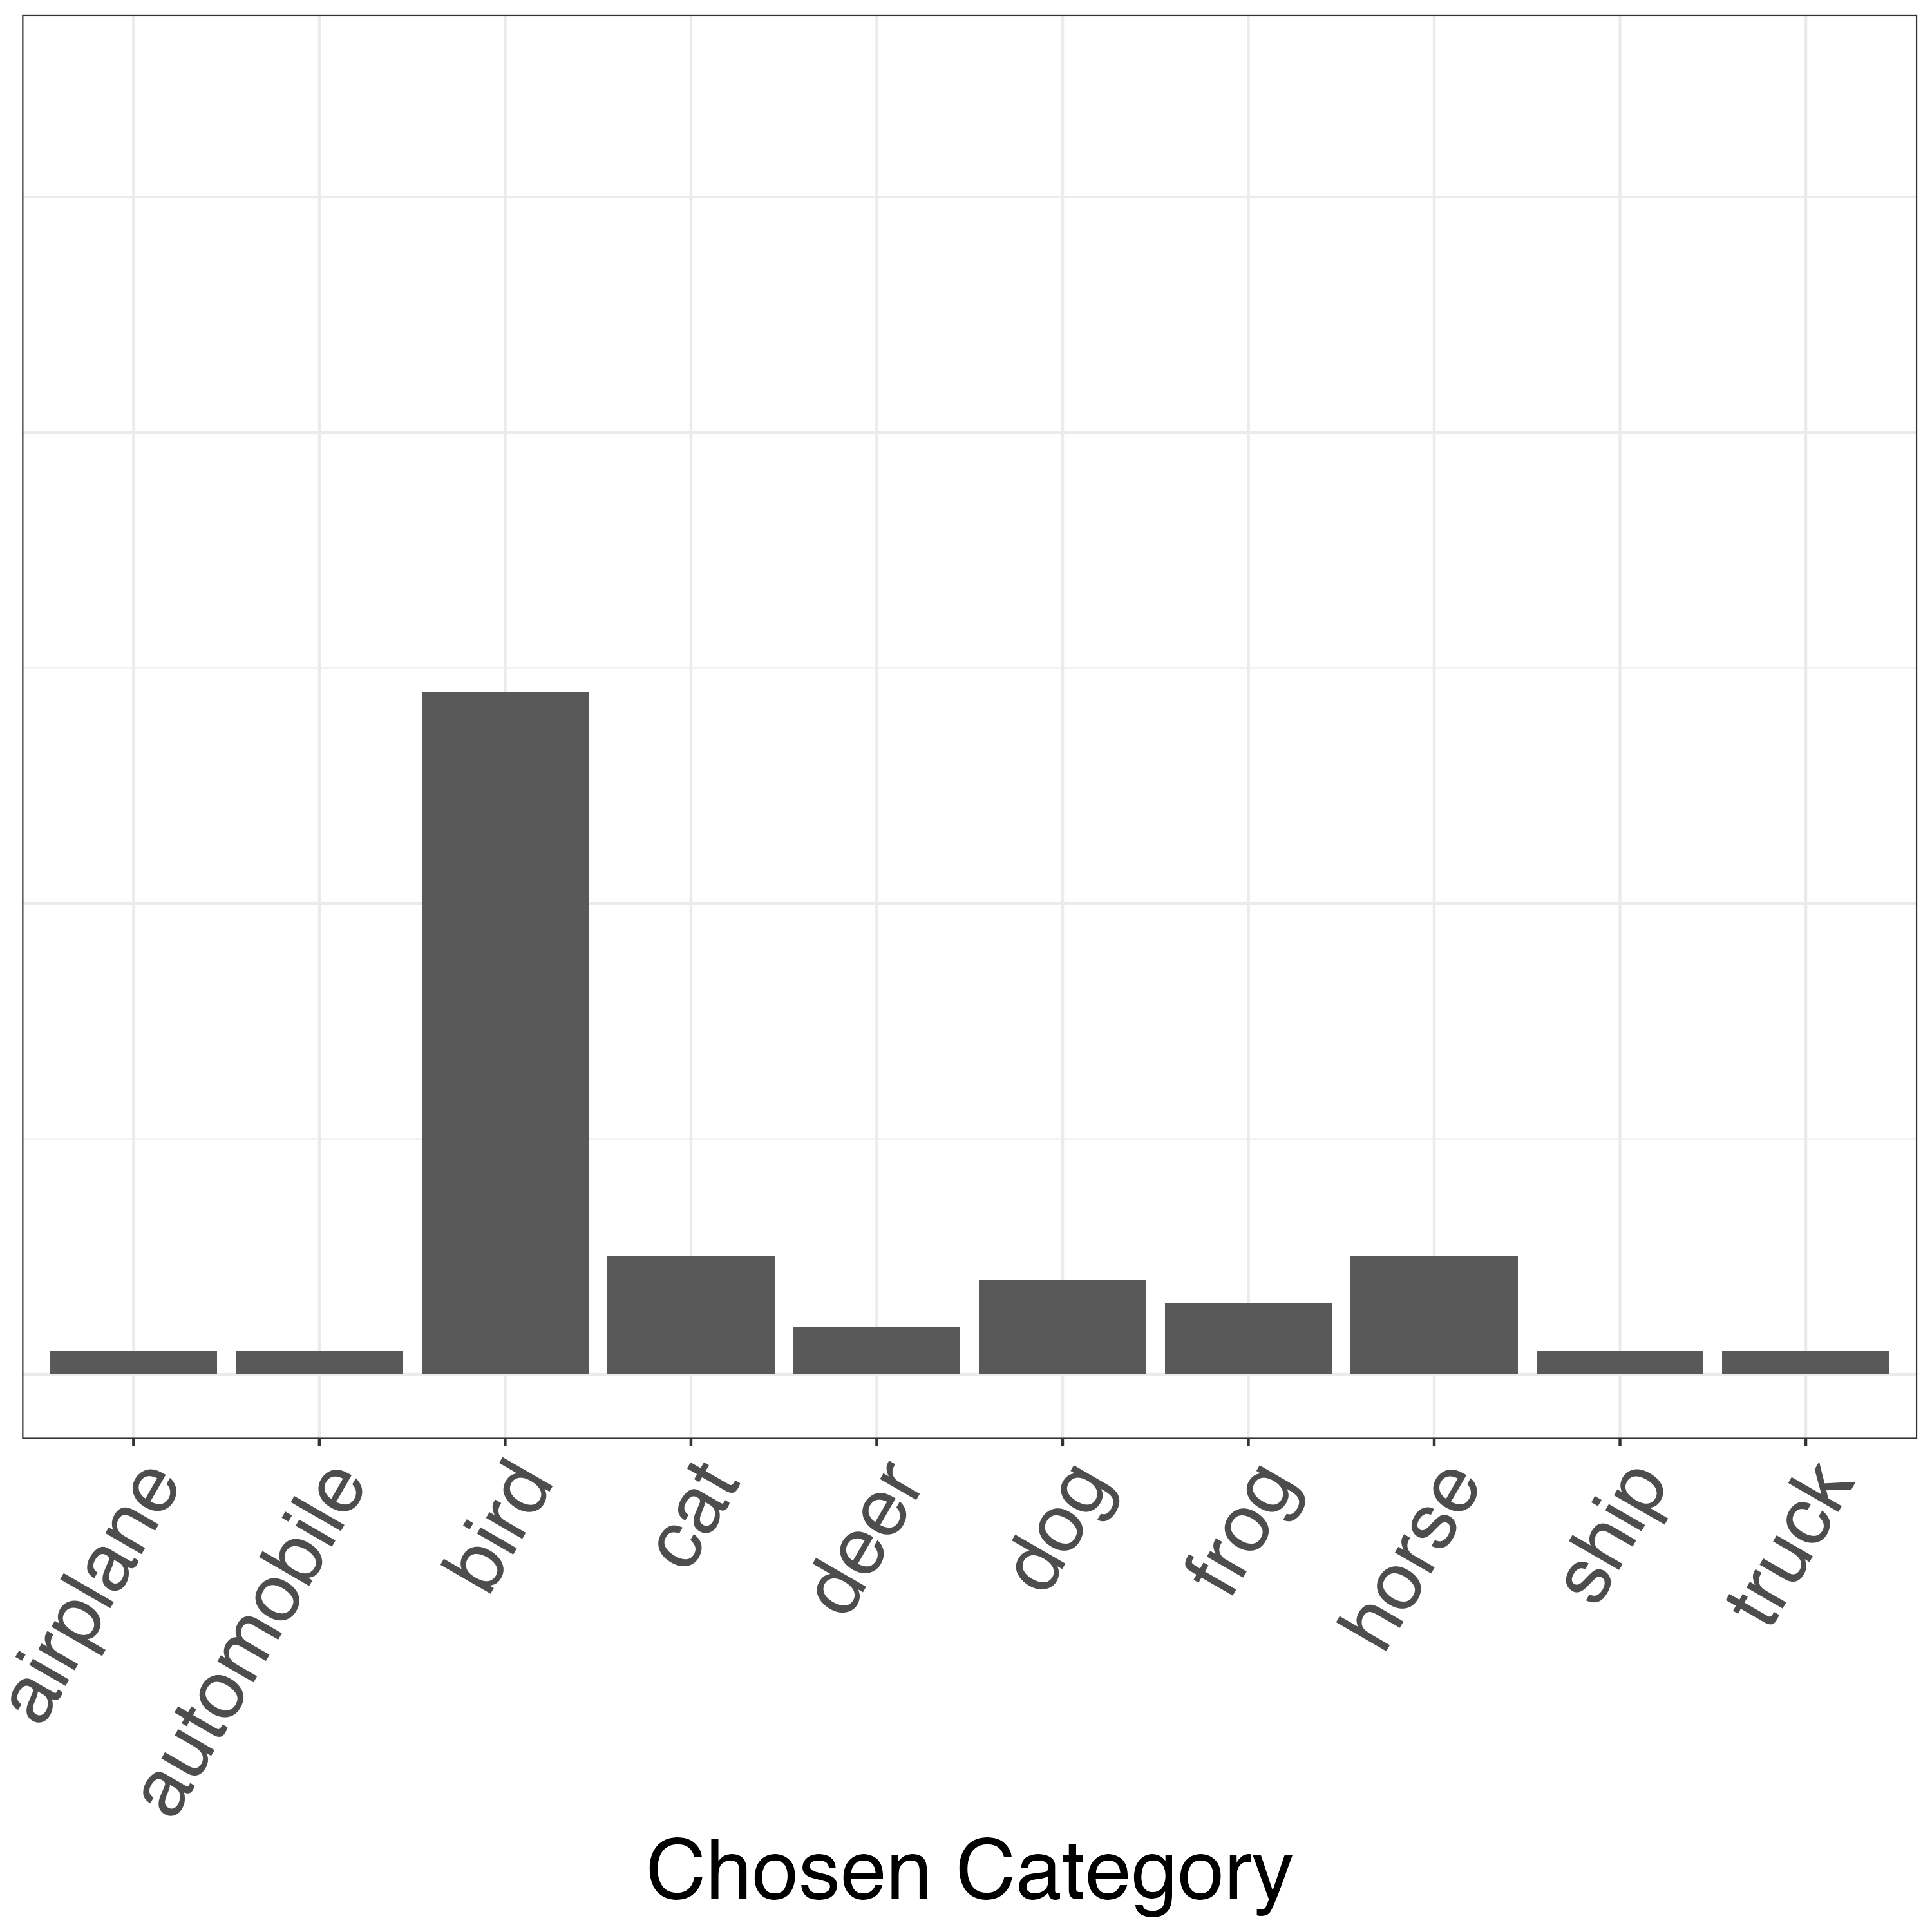
\includegraphics[width = 0.3\textwidth]{../figs/ambiguous_image2_dist.png} & 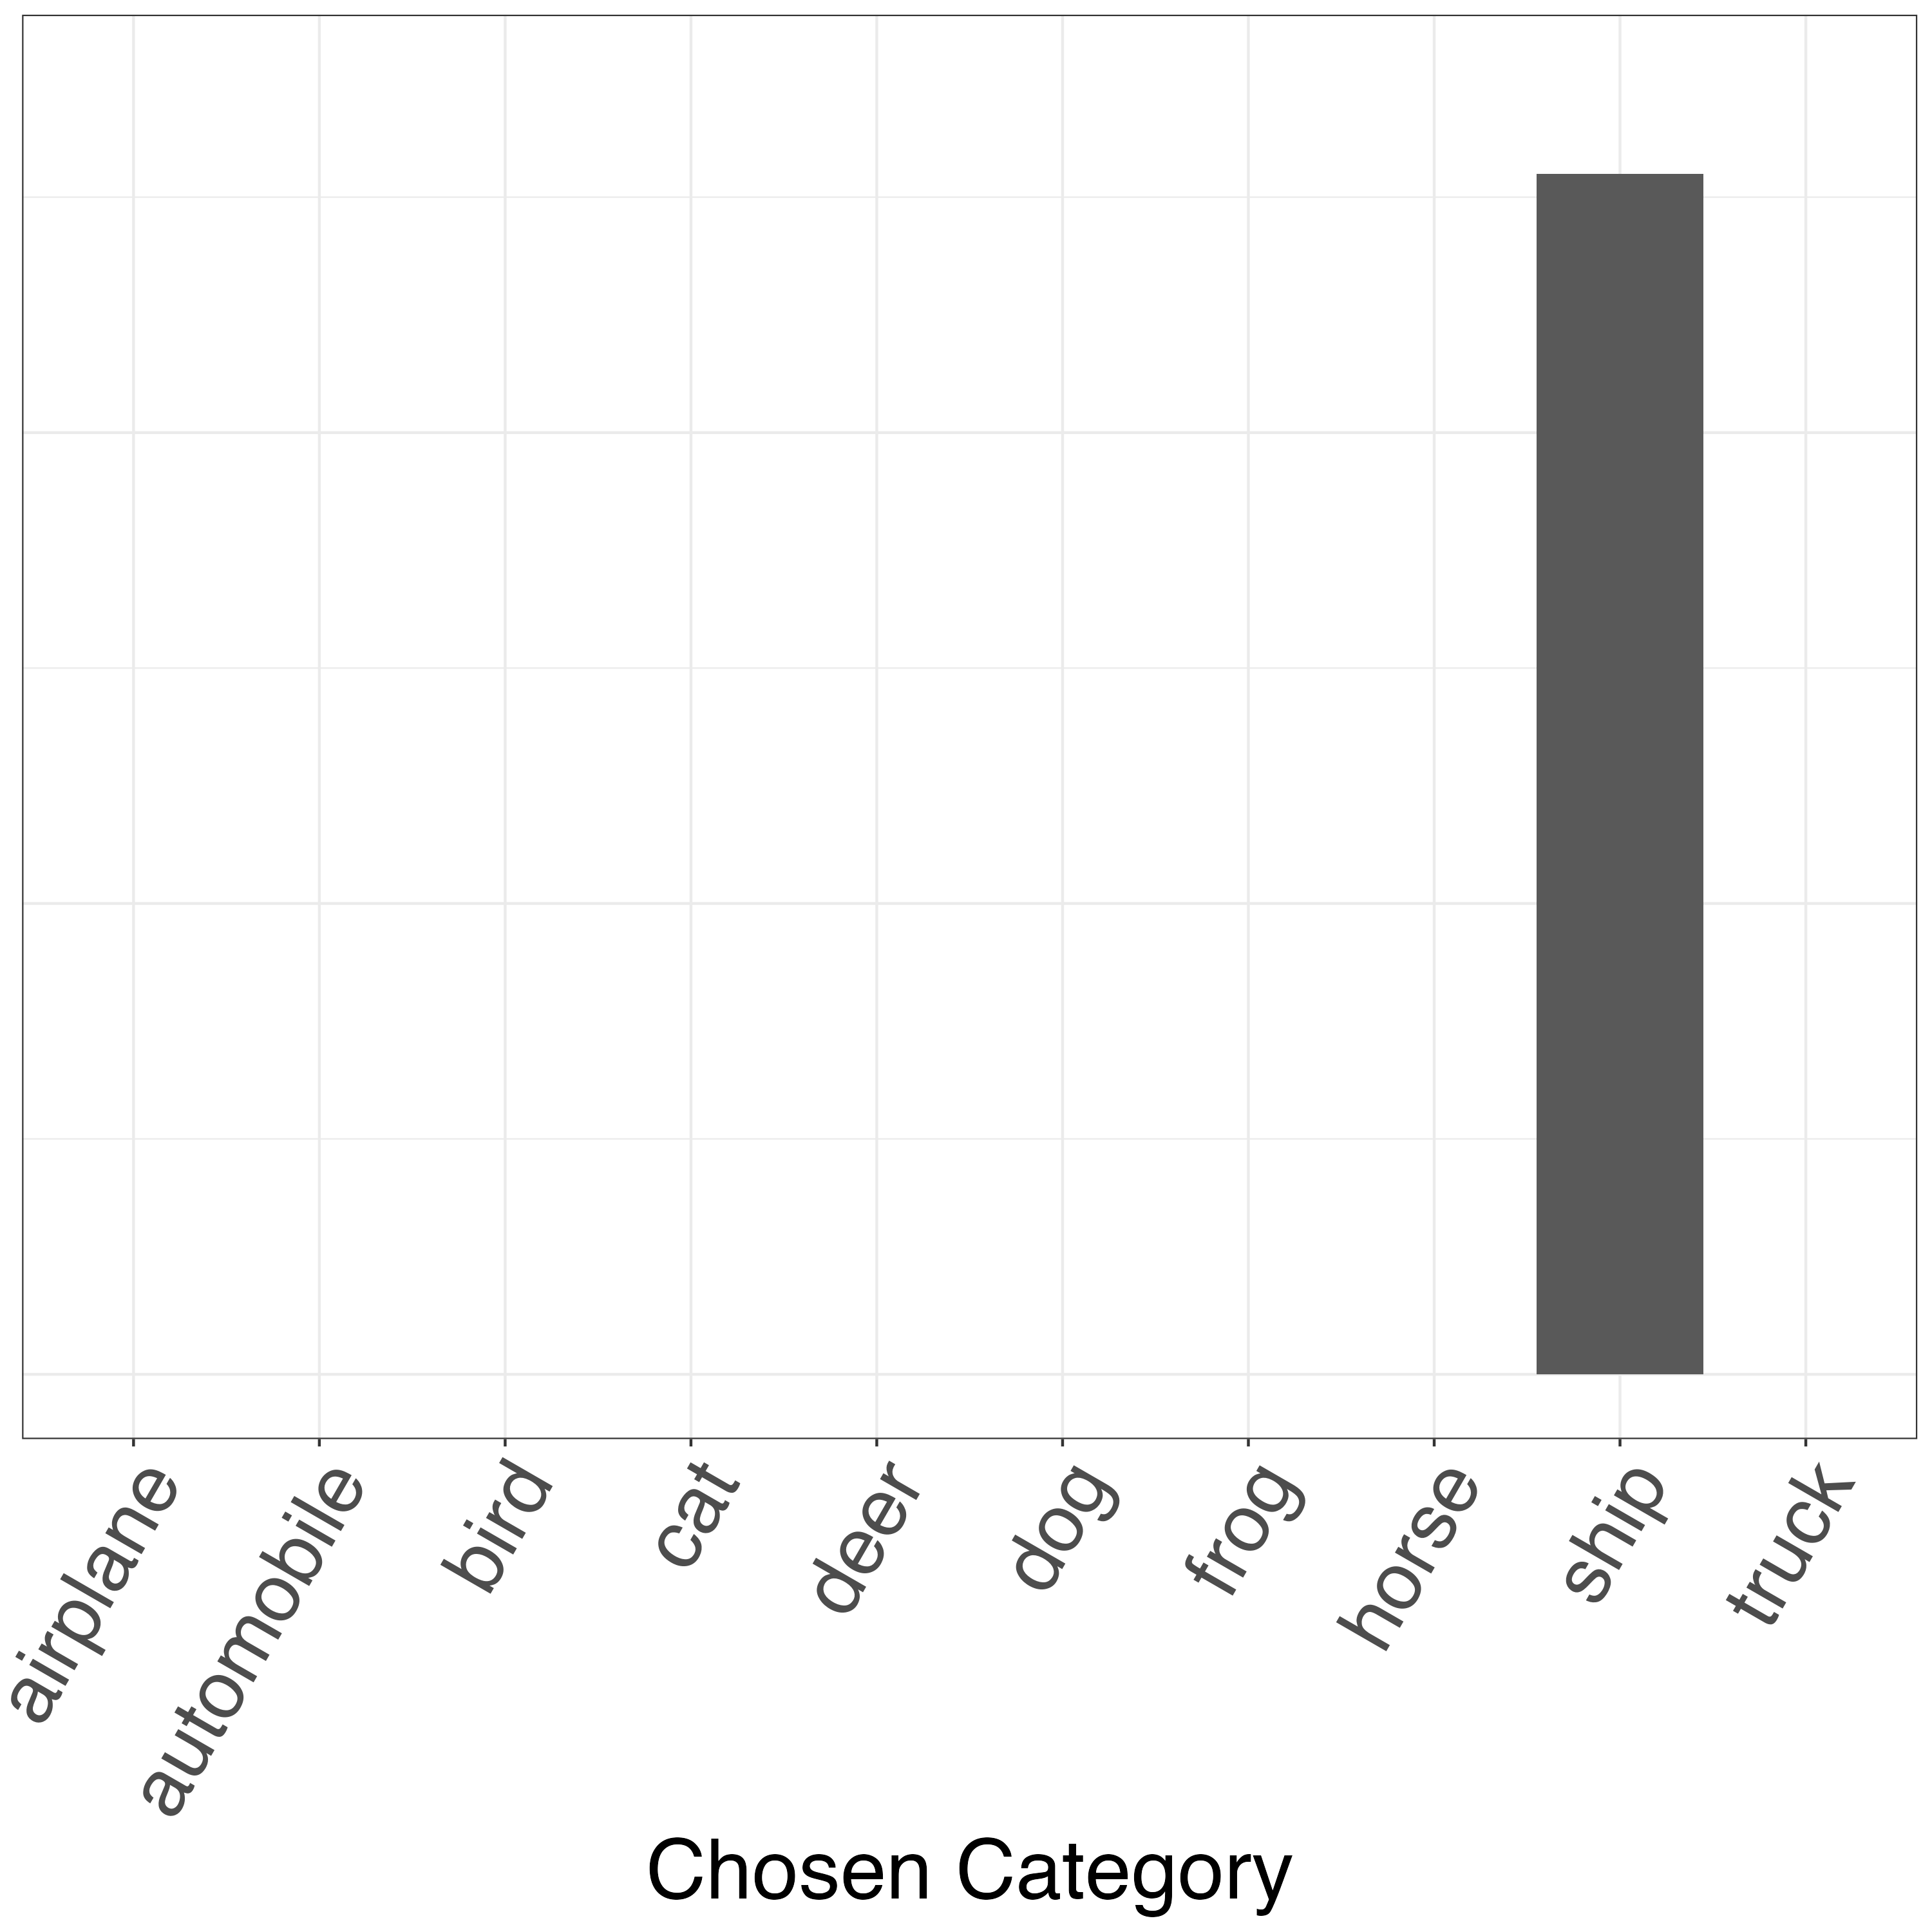
\includegraphics[width = 0.3\textwidth]{../figs/unambiguous_image_dist.png} \\
  \end{tabular}
  \caption{Example of an ambiguous image. The image shows a car, but the chosen
  categories are \textit{automobile} and \textit{truck}.}
  \label{fig:ambiguous_image}
\end{figure}